\chapter{Analyse der Ausgangssituation}\label{cha:ausgangssituation}
	Dieses Kapitel diskutiert die Motivation für die Abschlussarbeit, setzt klare Ziele sowie Rahmenbedingungen und erörtert den Einfluss des Java Modulsystems auf \textsc{Renew} wie auch die derzeitige Plugin-Architektur. Des Weiteren wird ein Zustand ermittelt, der als Basis für die nachfolgenden Prototypen gelten wird.

\section{Motivation}\label{sec:motivation}
	\textsc{Renew} ist ein Petrinetz Simulator, der von dem Arbeitsbereichs TGI entwickelt wird und unterstützt das Erforschen von komplexen Systemen auf der Grundlage formaler Modelle.\newline
	Weil \textsc{Renew} in Java geschrieben ist, ist die Applikation an die Java Plattform angewiesen und muss dementsprechend den Plattform Anforderungen und Richtlinien folgen. Die Anforderungen und Richtlinien sind nicht fix und können sich ändern, besonders mit einem großen Versionssprung. Das neu eingeführte Modulsystem von Java, wird mit einem großer Versionssprung in Verbindern gebracht und setzt neue Normen und Anforderungen für das Entwicklung von Java Applikationen. \bigbreak
	
	Es gibt mehrere Gründe warum \textsc{Renew} die Migration auf das Modulsystem durchführen sollte. Im Folgenden werden die wesentlichen Argumente, die für die Migration sprechen diskutiert.  

	\subsection{Architektur} \label{sub:architektur}
		Die initiale Entwicklung von \textsc{Renew} begann mit einer monolithischen Architektur. Diese erfüllte die nötigen Anforderungen, eignet sich jedoch nicht für Entwickler mit geringer Kenntnis über die Gesamtarchitektur und den darunterliegenden theoretischen Konzepten. Daher wurde eine Plugin-Architektur aufgesetzt, die es ermöglichte Studenten \textsc{Renew} mit Logik innerhalb eines Plugins zu erweitern. Dieses Verfahren trägt bereits den Gedanken der Modularisierung in sich, da die Gesamtarchitektur in Bestandsteile zerlegt und mit einander entkoppelt verknüpft wird. Somit wäre die Einführung des Modulsystems von Java der nächste Schritt in Richtung erweiterbare und zusammensetzbare Systeme.

	\subsection{Verkürzter Entwicklungszyklus}\label{sub:vez}
		Die Aufteilung einer monolithischen Architektur auf eine Plugin-Architektur war ein großes Ereignis für Renew. Denn mit der Zerlegung der Gesamtarchitektur, wurde die Komplexität auf die entstandenen Komponenten aufgeteilt und erlaubte eine mühelose Weiterentwicklung der Applikation über die Plugins. \bigbreak

		Obwohl die \textsc{Renew} Plugin-Architektur lange im Betrieb blieb, hatte das Plugin-System die Codebasis umorganisiert, ohne diese zu verändern. Diese führt zu altem, unverständlichem Code aus der Java 1.4 (2002) Version, mit dem viele Konzepte und Architektur Entscheidungen getroffen wurden. Nach fast 18 Jahren Betrieb altert die Codebasis, die Ideen und Konzepte für die Umsetzung ihrer Funktionalität. Besonders konfus und aufgebläht können Funktionsumsetzungen erscheinen, die heute von Java 12 in ein paar Zeilen gelöst werden können. Der zügige und rapide Wandel der Software Paradigmen und deren optimaler Einsatz in der Software Architektur ist ein Teil des Fortschritts und muss in die Planung des Lebenszyklus der Applikation mit einkalkuliert werden. \newline
		Dementsprechend ist die Modularisierung und dessen Anforderung an die Struktur und Inhalt ein wichtiges Ereignis für den \textsc{Renew} Lebenszyklus. Denn dieser erreicht wieder sein Ende und wird mit dem Modularisierungsschritt zurückgesetzt. \bigbreak

		\textsc{Renew}'s Entwicklungseinheit ist das Plugin. Diese repräsentiert ein bestimmtes Feature mit einem eigenen Lebenszyklus, wie zum Beispiel ein Formalismus, Simulator oder Fenster Management Plugin. Diese müssen Daten entgegennehmen, diese verarbeiten und wieder ausgeben. Demzufolge bündelt ein Plugin mehrere Fähigkeiten, die zusammen ein Feature verkörpern. Der wesentlicher Nachteil einer Codeänderungen in einem Plugin, ist das Beeinträchtigen des Gesamtverhaltens des Plugins und fordert dementsprechend ein komplettes Testszenario aller Plugin Fähigkeiten.\newline
		Mit der Einführung der Module, kann das Plugin in kleinere Einheiten zerlegt werden, die anschließend eine gekapselte Teilfunktionalität des Plugins in sich tragen und Auswirkungen der Modifikation eingrenzen. Diese sind klein, leicht änderbar, ersetzbar und besitzen einen eigenen unabhängigen Lebenszyklus. Somit verkürzt sich die Entwicklungsdauer einer Änderung innerhalb eines Plugins, da der Einfluss auf die Umgebung durch die Modulgenerzen eingeschränkt ist. Des Weiteren  bieten Module eine Möglichkeit kooperativ und parallel an einem Plugin zu arbeiten, indem die Module gegen vereinbarte Schnittstellenbeschreibungen entwickelt werden. \bigbreak

		Demnach erweitert die Modularisierung den \textsc{Renew} Kontext und erlaubt das Entwickeln von Plugins in Rahmen eines Studenten Projekts, indem Teilaufgaben eines Plugins auf Module zerlegt und parallel von Studenten bearbeitet werden können. Darüber hinaus ist das Zusammenführen der Ergebnisse eine konfliktfreie Angelegenheit und bedarf keiner kompletten Gruppenaufmerksamkeit, um die passenden Codeblöcke für die Gesamtfunktionalität auszuwählen, da es sich so gut wie keine Überschneidung in der Aufgaben Implementation bilden kann. Somit profitiert \textsc{Renew} von den kurzen Entwicklungszyklen der Module und deren unproblematischen Verknüpfungseigenschaften. 

	\subsection{Code-Bausteine}\label{sub:cbs}
		Eine der wichtigsten Fähigkeiten eines Entwicklers, ist die Beherrschung der Komplexität. Diese führt zu sauberem, lesbarem, wartbarem Code und erweitert den Lebenszyklus einer Software um ein Vielfaches. Um diese Kompetenz zu meistern, bietet das Modulsystem von Java unterstützende Werkzeuge, die den erstellten Code organisieren und strukturieren, um ein langlebiges Ergebnis zu erzielen.\bigbreak

		Da \textsc{Renew} das Produkt vieler Abschluss-, Projekt- und Promotionsarbeiten ist, durch die die Software ihre Gestalt annimmt, gibt es diverse Beschäftigte mit eigenen Zielen und Interessen. Daher ist eine allgegenwärtige, globale Strukturanforderung, die jedem Entwickler bekannt ist und die verpflichtend eingehalten werden muss, eine erstrebenswerte Charakteristik.\bigbreak

		Die im Kapitel \ref{cha:modularisierung} vorgestellten Modul Charakteristiken beschreiben die von dem Java Modulsystem eingesetzten Richtlinien für die saubere Softwareentwicklung und erzwingen zum Teil ein Still der fein granulierten Code-Bestandteile, die kombiniert ein Softwaresystem ergeben.\newline
		Die Charakteristiken fördern den Entwickler zum Entwickeln von abgeschlossen Einheiten auf und verhindern somit das Entstehen von den sogenannten \textit{Spaghetti Code}, der funktionsübergreifende Anpassungen trifft und den Überblick über den Zusammenhang der Gesamtarchitektur unscharf erscheinen lässt. \bigbreak

		Die Module und die entsprechenden Richtlinien erschweren den \textit{Spaghetti Code}, indem Mehraufwand für die Kommunikation zwischen den Modulen erbracht werden muss und machen das unsaubere Arbeiten unattraktiv. Somit dienen Module als Grenzen für den Entwicklungsrahmen eines Features und engen den Bearbeitungs- und Betrachtungsraum für den Entwickler ein. Daraus ergibt sich ein Softwarepaket, das unabhängig von den Senior-Entwicklern verstanden, genutzt und angepasst werden kann, da der Aufbau nicht mehr in dem Wiki, Readme oder beim Entwickler selbst verankert, sondern direkt in der Codebasis integriert ist.\bigbreak

		Demzufolge profitiert \textsc{Renew} von der Modularisierung, indem sich immerfort wechselnden Akteure eine saubere Codebasis hinterlassen, die den nächsten Absolventen sowie den wissenschaftlichen Mitarbeitern viel Zeit erspart. \bigbreak

		Aus einer sauberen Umsetzung folgen saubere Code-Bausteine, die wiederverwendet werden können. Die genannten Eigenschaften der Module bringen einen wesentlichen Vorteil beim Optimieren der \textsc{Renew} Applikation, indem kontextbezogen Module ausgetauscht werden können, um ein besseres, lokales Ergebnis zu erzielen. Zum Beispiel können zielgerichtet ausgewählte Plugins für die Erfüllung einer speziellen Aufgabe, wie das Validieren von P/T-Netzen, ein besseres Ergebnis abliefern, indem ein für diesen Anwendungsfall angepasste Verarbeitungsalgorithmus angewandt wird. Dieser ist natürlich in einem Modul gekapselt und besitzt Schnittstein identisch zu seinem Vorgänger. Auf diese Weise kann eine große Anzahl an Modulen mit gleicher Funktion und unterschiedlicher Zielsetzung erstellt werden, die in einem Modulkatalog verwaltet und bei Bedarf ausgetauscht werden können.

	\subsection{Code Management} \label{sub:code_managment}
		Das Plugin Management ist ein zentrales Themengebiet von \textsc{Renew}, da Plugins geladen instanziirt und genutzt werden müssen. Diese wichtige Aufgabe übernimmt der \textit{PluginManger} innerhalb des \textit{Loader} Plugins, der Plugins in den Klassenpfad lädt und mit den benötigten Bibliotheken ausstattet. Das Ladend geschieht über den Plugin Classloader, der den Code aus aus den gegebenen Quellen auf den Klassenpfad platziert.\bigbreak
		\begin{figure}[t]
		  \centering
		  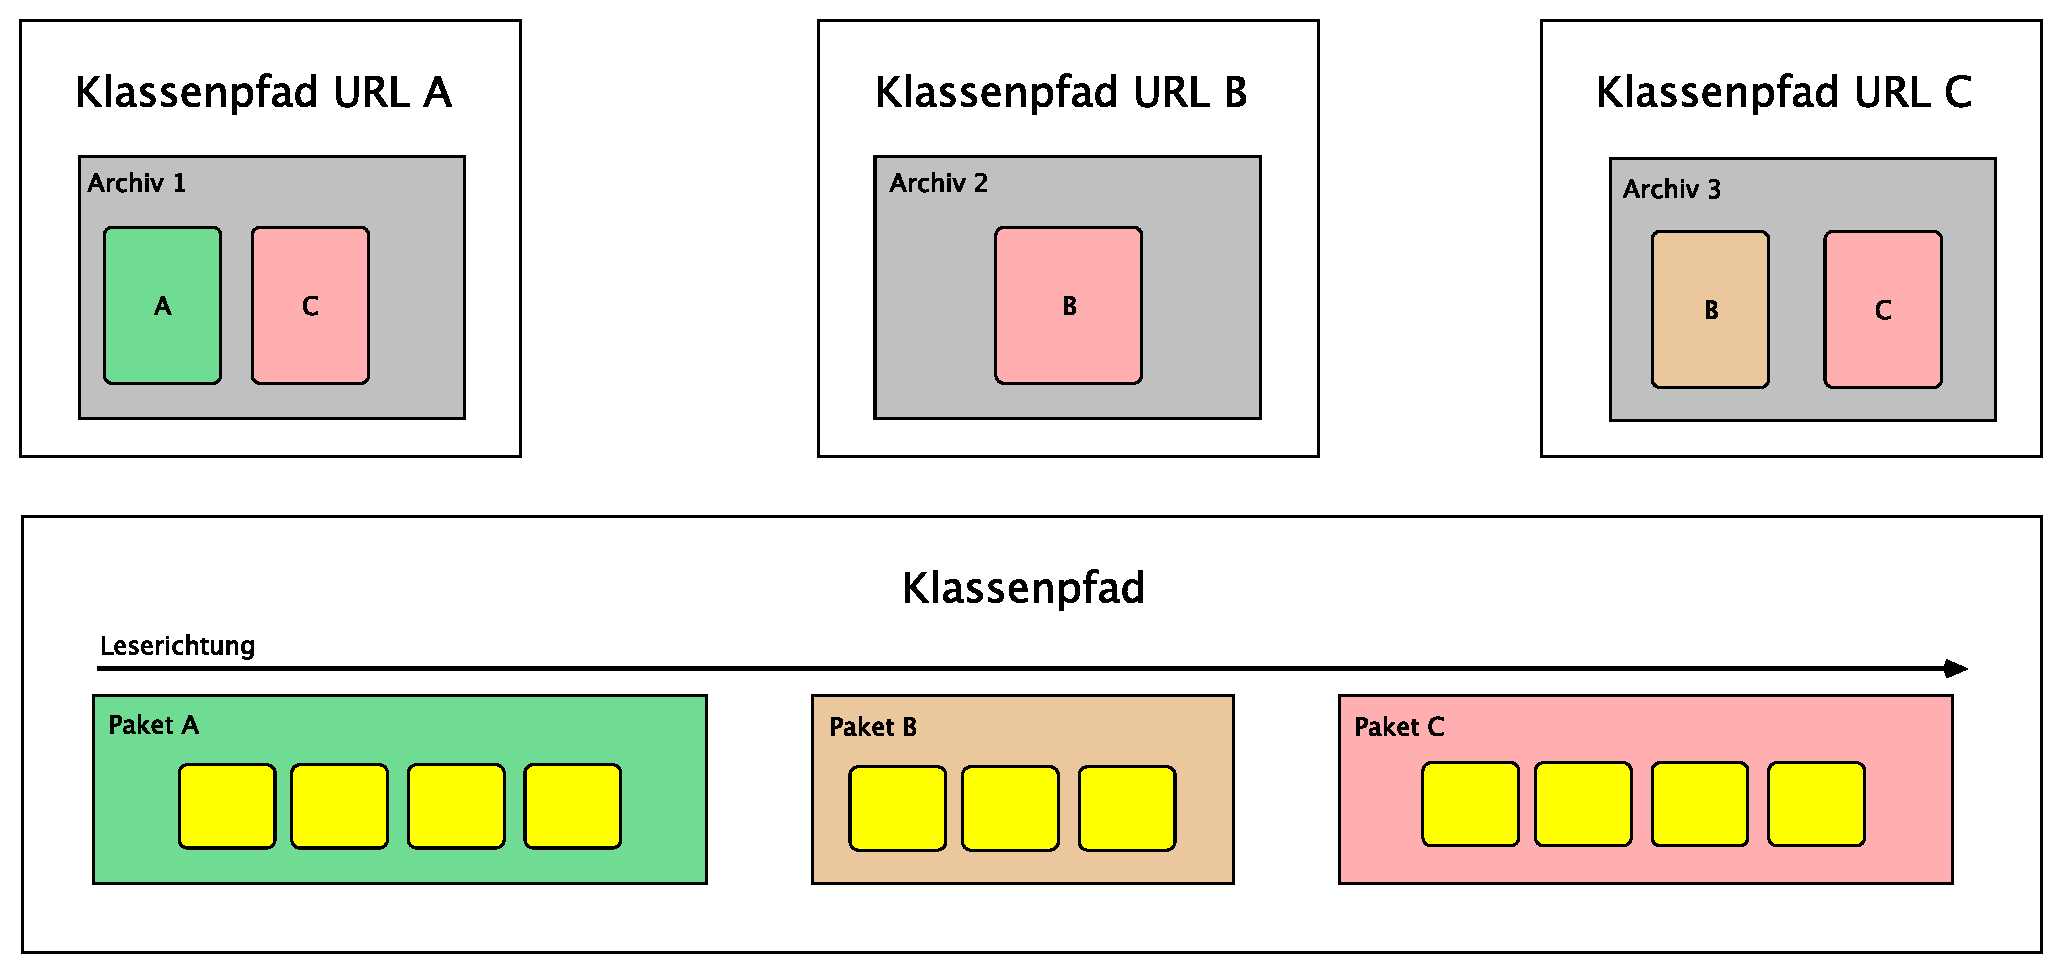
\includegraphics[width=\textwidth]{material/images/Klassenpfad.pdf}
		  \caption{Klassenpfad Suche}
		  \label{fig:CP_Struktur}
		\end{figure}
		Der große Nachteil des Klassenpfad, ist die Auflösung von Archiv Grenzen und somit auch von Plugin Grenzen. Das heißt, Java kann nicht unterscheiden aus welcher Bibliothek die Klasse stammt und muss aus diesem Grund den kompletten Klassenpfad für eine Plugin Klassenabfrage durchsuchen. Infolgedessen ist das Überwachen der Plugins auf dem Klassenpfad nur schwer möglich, da der Klassenpfad nur Informationen über die Klassen und ihre Pakete besitzt \ref{fig:CP_Struktur}. Des Weiteren ist die Zuordnung einer Klasse zu ihrer Quellen ebenso Problematisch.\bigbreak

		Dieses Verfahren wurde ständig bemängelt und wird mit der Einführung des Modulsystems von Java adressiert, indem die Konfigurationsdateien \textit{module-info.java} eingeführt wurde, die der Klassen Quelle eine Identität verleiht. Demzufolge ist ein Archiv oder Verzeichnis nicht mehr ein aussagen loser Behälter, sonder ein Objekt, das Information über seine Kennung, seinen Inhalt und seiner Kommunikationspartner besitzt.\newline
		Dies bring zwei wesentliche Vorteile für die Arbeit mit dem Plugin Code. Die erste Eigenschaft beschreibt Referenzen auf Archiv-Objekte, die die benötigte Klassen besitzen. Der Klassenpfad wird nicht mehr von links nach rechts durchsucht \ref{fig:CP_Struktur}, sondern über das Modul mit den entsprechend Klassen adressiert \ref{fig:MP_Struktur}. \newline
		Das bewusste Nachschlagen nach Klassen erhöht die Performance und setzt zusätzlich das eindeutige und verantwortliche Modul für die gegebene Implementation fest. Darüber hinaus erleichtert die eindeutige Modulzuordnung das Verfolgen von unerwarteten Verhalten, wie zum Beispiel das Überdecken von Klassen von weiteren Klassen des selben Typs, die sich weiter vorne im Klassenpfad befinden.\bigbreak 
		\begin{figure}[h!]
		  \centering
		  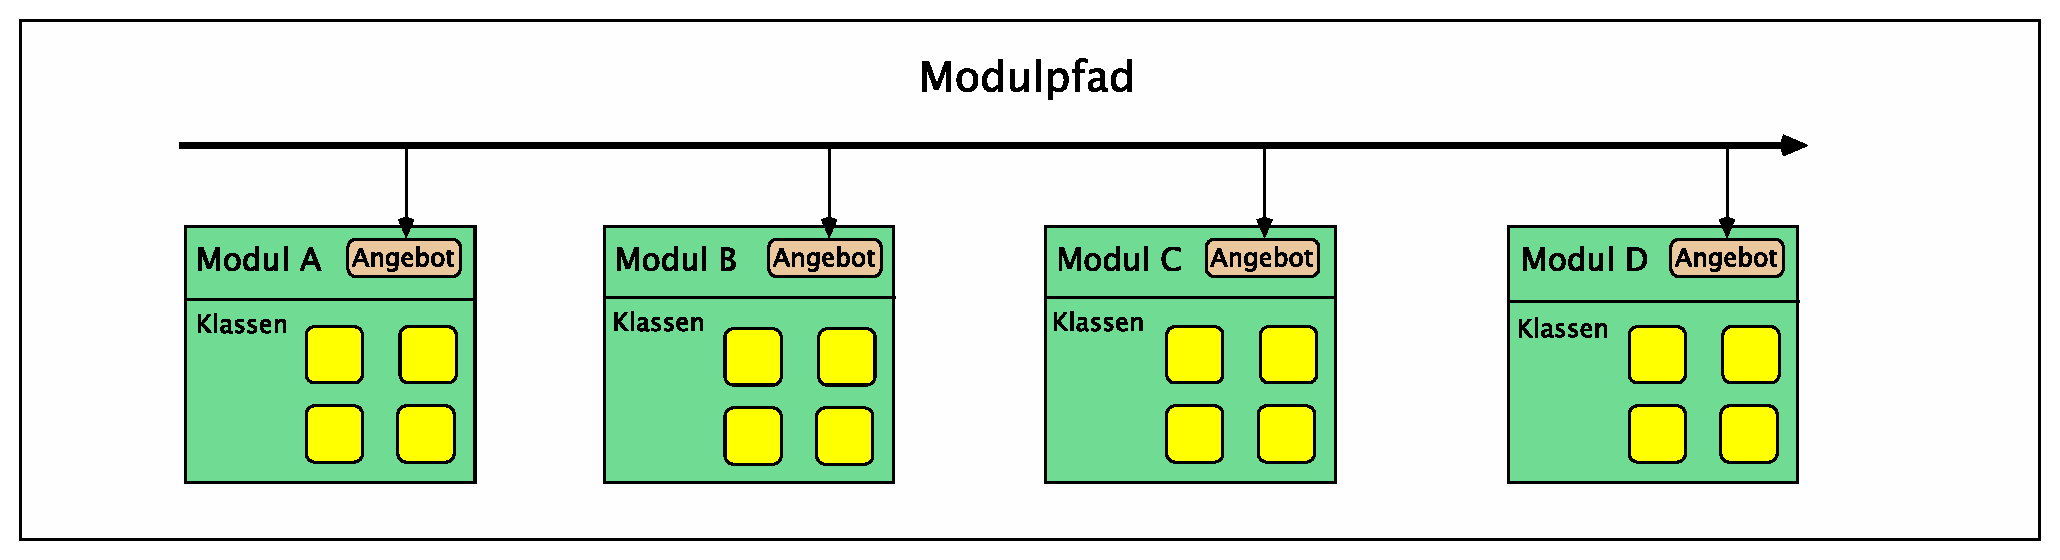
\includegraphics[width=\textwidth]{material/images/Modulpfad.pdf}
		  \caption{Modulpfad Suche}
		  \label{fig:MP_Struktur}
		\end{figure}
		Der zweite Vorteil, beschreibt das Auslesen der Modulinformation aller Module die sich auf den Modulpfad befinden. Demzufolge können Plugins in Archive verpackt und auf dem Modulpfad wieder gefunden, analysiert und sogar bearbeitet werden. Somit bring Java ein neues Instrument zum Verwalten der Codebasis von modularisierten Anwendungen, die dem Nutzer bei Bedarf die internen Bausteine präsentieren lässt.\bigbreak

		\textsc{Renew} kann mithilfe der neuen Modul API die Verwaltung der Plugins erweitern, indem geladenen Plugins direkt angesprochen und manipuliert werden. Zum Beispiel könnten auserwählte Plugins nur für bestimmte Nutzer oder Modi ihre Funktionalität anbieten oder eine angenehme Visualisierung der laufenden Plugins und dazugehörige Funktionalitäten dem Nutzer präsentieren. Des Weiteren ist die performante Suche nach Klassen in einem dynamischen System wie \textsc{Renew}, eine erstrebenswerte Qualität.  \newline
		In folgenden Kapitel der Auswirkungen \ref{sec:auswirkung} wird auf die \textit{ModulLayer} eingegangen, die das zielorientierte Laden nur notwendiger Module und somit nur notwendiger Plugins ermöglicht.

	\subsection{Laufzeit-Abbildung} \label{sub:laufzeit_images}
		Für die Nutzung von Java Applikationen ist immer ein installierte Laufzeitumgebung notwendig, die Versionskompatibel mit der entsprechenden Applikation sein muss. Dementsprechend muss Java installiert und eingerichtet werden bevor unser Code ausgeführt werden kann. Für große Serveranwendungen ist der Aufwand gerechtfertigt, da diese unikale, langlebige und komplexe Gebilde sind. Für Anwendungen die kleiner sind und dynamisch zwischen Hardwareknoten verteilt werden müssen, ist das manuelle Anlegen der Laufzeitumgebung eine mühselige und fehleranfällige Aufgabe. \newline
		Das Modulsystem von Java hat diese Herausforderung mithilfe der \textit{Laufzeit-Abbildung} adressiert. Die \textit{Laufzeit-Abbildung} besteht aus einer Verzeichnis Struktur, die alle notwendigen Komponenten für den Betrieb der Applikation besitzt. Dazu zählen Module, Skripte, native Bibliotheken, Konfigurationen, Dokumentationen sowie Lizenzbedingungen und sogar Sicherheitsmechanismen zum Validieren der Komponenten sind vorgesehen. Die generierten \textit{Laufzeit-Abbildungen} sind in sich Abgeschlossen und können einfach auf beliebig viele Hardwareknoten automatisiert verteilt und ausgeführt werden, ohne zusätzliche Justierung der Software Umgebung. \bigbreak
		Die Eigenschaft der Abgeschlossenheit der \textit{Laufzeit-Abbildung}, kann von \textsc{Renew} aufgegriffen und genutzt werden, um ausgewählte Plugin Gruppen horizontal nach belieben zu skalieren. Zusätzlich hält die \textit{Laufzeit-Abbildung} nur notwendige Java sowie Benutzer erstellte Module, die bestens für die Ausführung der Applikation auf einander abgestimmt werden. Infolgedessen kann das modularisierte \textsc{Renew} auf optimale Ausführungsgeschwindigkeiten zählen. 

	\subsection{Vision} \label{sub:moderner_zustand}
		% Ziel
		Der zeitgemäße Zustand einer Applikation ist ein Zeichen hoher Qualität und reflektiert enorme Ansprüche an den Betrieb der Applikation. Diese kann geschäftskritische Qualitäten tragen, die den marktführenden Vorteil bringt und der Konkurrenz ein Schritt voraus ist. Um den Vorsprung zu sichern, ist eine vorausschauende Flexibilität gefragt. Mithilfe dessen die Applikation in der Lage ist, mit minimalem Aufwand, an die führenden Technologien anzuknüpfen. 

		% Trends 
		Die aktuell führenden Trends beschäftigen sich mit der verteilten und wiederverwendbaren Softwareumsetzungen, die ständig an Komplexität gewinnen und trotzdem leicht beherrschbar bleiben muss. Diese beschreiben Ansätze wie gewisse Ziele erreicht werden können und setzen Grundvoraussetzungen zum Erreichen dieser Ziele. Dementsprechend muss \textsc{Renew} bestimmte Grundvoraussetzungen erfüllen, um die Vorteile der Trends zu Nutzen und den Schritt mit dem Fortschritt zu halten.  \bigbreak

		% Docker  
		Zum Beispiel wäre die Docker Umgebung für \textsc{Renew} eine willkommene Erweiterung, mit der interne Bestandsteile distributiv betrieben werden können. Somit wäre die Ausführung von \textsc{Renew} nicht mehr an eine Maschine gebunden und kann bei Bedarf horizontal skaliert werden. Im Folgenden stellt sich die Frage: welche internen Strukturen von \textsc{Renew} müssen individuell behandelt und anschließend kooperativ zusammengeführt werden. Auf diese Frage gibt es keine pauschale Antwort, jedoch ist es klar, dass die Plugins von \textsc{Renew} feingranular betrachtet werden müssen, um sich ein Bild der Verarbeitungskette zu erstellen und diese den Bedürfnissen anzupassen. \bigbreak

		% Microservice  
		\textsc{Renew} auf verschieden Hardwareknoten zu verteilen ist nur der erste Schritt der distributiven Ausführung. Es fehlt die Koordination zwischen den Knoten, die die Verarbeitung koordinieren und die Ergebnisse zusammenfassen. Somit gibt es eine weitere Technologie, die sich dieser Aufgabenstellung widmet: Der Mikroservice Architekturansatz, der sich um die Koordination und das Zusammenspiele von Applikationsschwärmen kümmert. \bigbreak

		% Fazit 	
		Mithilfe der Mikroservicearchitektur und der Docker-Umgebung wäre die distributive Ausführung von \textsc{Renew} erreichbar, doch zuerst muss \textsc{Renew} den aktuellen Stand der Technologie entsprechen und demzufolge das Modulsystem von Java integrieren.  

\section{Folgen} \label{sec:auswirkung}
	Die Folgeerscheinung der Modularisierung unterbindet zahlreiche Entwicklungsschwächen, wie die \textit{Code Organisation}, \textit{Zyklen}, \textit{Split Packages} und antiquierte API's. Diese sollen mit der Migration auf das Modulsystem von Java aufgelöst, reorganisiert und nachgerüstet werden, um einen kompelierfähigen Zustand erreichen zu können.

	\subsection{Projektstruktur} \label{sub:projektstrukutr}
		Das Plugin System von \textsc{Renew} besteht aus einer großen Anzahl an Plugins, die Zweckorienttier kombiniert werden können. Demnach besteht bereits ein Organisationsaufwand, der mit jeder Plugin Kombination wächst. Zu den bestehenden Organisationsaufwand wird zusätzlich eine neue Ebene der Administration eingeführt, nämlich die Ebene der Module. Diese zerlegen Aufgabenmengen aus einer Code-Struktur in mehrere Code-Bausteine, die infolgedessen disjunkt verwaltet werde müssen.\newline
		Die Verwaltung von Plugins und ihrer Module ist eine wichtige und verantwortungsvolle Aufgabe, die für divergierte \textsc{Renew} Anwendungsfälle unterschiedliche Kombinationen von Plugins und der entsprechenden Module zuständig sein wird.\newline
		Dementsprechend muss eine passende Projektorganisation eingerichtet werden, die jedem Plugin die Möglichkeit bietet zusätzliche Module, mit dem Quell-Code, den Ressourcen sowie den Tests, zu erstellen.\bigbreak
		Des Weiteren spielt die Paket Organisation eine zuzunehmend stärkere Rolle im Modulsystem von Java, denn eine Überschneidung eines Paketnamens mit anderen Bibliotheken im System ist ausgeschlossen und muss dementsprechend einen global eindeutigen Namen besitzen. \newline
		Die Einschränkung in der Namensgebung und Code Organisation ist für \textdc{Renew} eine substantielle Änderung. Die Plugins wurden von unterschiedlichen Entwickler zu unterschiedlichen Zeitpunkten entwickelt, ohne eine einheitliche Struktur Plugin übergreifend einzuhalten. Daraus folgt eine wilde Resourcen- und Java Fremdcode Allokation, die das Lesen, Analysieren und bearbeiten der Plugins schwierig gestaltet. Zum Beispiel befinden sich gewisse Ressourcen im Plugin Wurzelverzeichnis unter \textit{tools}, \textit{samples}, \textit{ontology} und andere direkt im Java Source-Code unter \textit{src/**/*.(gif|jj|rnw|sns|vm)}. Der Aufbau führt zu der Frage, wie kompatibel ist das Ressourcen Layout mit dem Modulsystem von Java. Denn, Ressourcen sowie Klassen werden innerhalb eines Pakets im Modulsystem von Java gleich behandelt und gekapselt. Demzufolge kann das Paket \textit{samples} nur ein mal in der Modulmenge geben, da ein Modul global den Kompletten Namensraum für sich und seine Ressourcen allokiert. \bigbreak 

		Das Problem der Ressourcenorganisation, kann mithilfe des \textit{META-INF} Verzeichnis gelöst werden, indem alle benötigten Ressourcen wie Konfigurationsdateien, Bilder und komplexe Darstellungsobjekte in dieses Verzeichnis verschoben werden. Das \textit{META-INF} Verzeichnis ist ein besonderes Verzeichnis, das nicht als ein Klassenpaket interpretiert wird und dementsprechend keinen ausführbaren Code enthält. Demzufolge können namensgleiche Ressourcen und Paketstrukturen in unterschiedlichen Modulen den selben Namensraum besetzen. \bigbreak

	\subsection{Split Packages}
		Im Kapitel \ref{sub:code_managment}  wurde die neue Klassensuche innerhalb des Modulsystems von Java thematisiert. Die Klassensuche ordnet jedes Klassenpaket eindeutig einem Modul zu, um den Klassenpfad durch eine Struktur zu erweitern, die Sicher, Schnell und Eindeutig ist. Für \textsc{Renew} ist die Voraussetzung der eindeutigen Paketbenennung nicht erfüllt. Denn, \textsc{Renew} besteht aus Plugins, die sich gegenseitig sowohl ergänzen als auch erweitern und neigen dementsprechend zum ähnlichem oder äquivalentem Aufbau. Zum einen geschieht es bedacht, um zusammengehörige Klassen auf dem Klassenpfad näher zu bringen und unter einem Paketnamen zu vereinen, zum anderen geschieht es zufällig, da sich der Aufbau gut für die Zielsetzung eignet.\bigbreak

		Die Lösung für das Problem ist die Anpassung der Paketstruktur, die eindeutig für jedes Plugin definiert wird. Zum Beispiel müssen Plugins aus dem gleichen Kontext, wie \textit{Navigator} oder \textit{NavigatorGit}, die den selben \textit{de.renew.navigator.*} Namensraum beanspruchen disjunkt aufgebaut und benannt werden, um eine eindeutige Identität zu etablieren. \bigbreak

		Das erweitern von Plugins, indem gleichnamige Paketstrukturen aufgebaut werden, ist ein Komplexes und tief führendes Problem. Wie bereits im Kapitel \ref{sub:projektstrukutr} besprochen, darf es keine Überschneidung der Namensräume geben. Das heißt, die  Annahme, dass die benötigten Klassen aus anderen Plugins sich in dem selben Paket auf dem Klassenpfad befinden ist nicht mehr zutreffend. \newline
		Für \textsc{Renew} hat es eine ganz besondere Bedeutung, da der Code nicht nur Kompiliert sonder zuvor generiert werden muss. Das generieren geschieht mit unterschiedlichen Techniken, die mit \textit{rnw, sns, jj, mv} Dateiformaten arbeiten und für bestimmte Anwendungsfälle unterschiedliche Java Klassen sowie Ressourcen generieren. Der Code und die Ressourcen orientiert sich auf das Zielpaket und nutzt zum Teil keine \textit{imports}, sondern direkte Klassen Zugriffe, da man sich sicher ist, dass die benötigten Klassen von anderen Plugins innerhalb ihres Pakets nachgeladen werden.\bigbreak

		Das Problem der \textit{Split Packages} beginnt im Kontext der \textsc{Renew} Generatoren. Diese generieren nicht nur Java Klassen spezifisch für einen Anwendungsfall, sondern auch Ressourcen, die in unterschiedlichen Szenarien eingesetzt werden. 
		Dementsprechend liegt das Problem nicht in der Java Klasse oder dem Plugin, sonder in der Verarbeitungskette der Generatoren, die variable Java Klassen sowie dazu passende Ressourcen erstellen. \newline
		Um die \textit{Split Packages} aufzulösen, müssen die Verarbeitungsketten von vorne bis hinten Analysiert und angepasst werden. Dazu zählt das Auffinden der benötigten Java Klassen innerhalb der modularisierten Plugin Menge, das Verweisen auf den vollwertigen Klassen Namen sowie das Öffnen und Konsumieren der entsprechender Pakete aus den notwendigen Plugins. Des Weiteren muss der Anwender der Ressourcen den vollen Zugriff auf alle in der Ressource referenzierten Klassen besitzen, um dessen Inhalt darstellen zu können.\bigbreak

		Das Einsetzen der \textit{Split Packages}, ermöglichte den Entwickler eine einfache Art und Weise Code aus unterschiedlichen Quellen zusammenzuführen. Jedoch hat sich die Technik auf lange Sicht nicht bewährt und wird mit dem Modulsystem von Java entfernt. Da \textsc{Renew} über einen langen Lebenszyklus verfügt und diese Technik von Beginn an weitgreifend einsetzte, müssen diese Mängel behoben werden bevor \textsc{Renew} auf den Modulpfad Einsatzbereit ist. 

	\subsection{Projekt Verwaltung} \label{sub:verwaltung} % gradle tiefer erklären 
		Die Herausforderung dynamische Modulkombination aus einer großen Modulmenge zu erstellen, spielt eine zentrale Rolle in einem Modulverband. Daher ist die Administration ein wichtiges Instrument für das Entwickeln von Modularem Code.\newline
		Für die Verwaltung der Codebasis existieren bereits Werkzeuge wie \textit{Ant}, \textit{Maven} und \textit{Gradle}, die eingesetzt werden können. Da \textit{Gradle} das zurzeit aufstrebende Software Instrument für das erstellen von ausführbaren Software Artefakten ist und die besten Eigenschaften von \textit{Maven} sowie \textit{Ant} in sich vereint, ist dieses bestens für das Modulsystem gewappnet und sollte im \textsc{Renew} Kontext eingesetzt werden. \bigbreak
	    Die zentrale Aufgabe von \textit{Gradle} besteht aus dem Bauen von kompatiblen Plugins mit den geeigneten Modulen, die über Konfigurationsdateien, Benutzereingaben, und äußeren Einflüssen gesteuert und ausgeführt werden sollten.

	\subsection{Homogene Umgebung} % plugin.cfg vergleich
		Ein weit verbreitetes Problem der Softwareentwicklung, ist der Unterschied der Laufzeit- sowie Entwicklungsumgebung. Die Entwickler arbeiten auf einer bestens eingerichteten Maschine mit allen nötigen Bibliotheken und Abhängigkeit, die in der Zielumgebung zu meist nicht existieren. Um der Diskrepanz des Ausführungskontextes entgegen zu wirken, wird eine Richtlinie benötigt, die den Kontext einer Applikation beschreibt. Aus diesem Grund deklariert die \textit{module-info.java} eine globale Plattformunabhängige Anforderung an benötigten Modulen und Bibliotheken, die zu der Kompilations- sowie Ausführungszeit präsent sein müssen.\bigbreak

		Die \textsc{Renew} \textit{plugin.cfg} erfüllt die Funktion einer Richtlinie der benötigten zugrunde liegender Plugins, jedoch fehlen die Deklaration der unterstützenden Bibliotheken, die für die Ausführung von \textsc{Renew} benötigt werden. Daher ist die explizite Deklaration der notwendigen Drittanbieter-Bibliotheken wie \textit{log4j} eine willkommene Erweiterung für Renew. 


	\subsection{Schnittstellen} % erweiterung auf kapselung der internen struktur , es giebt viel gemeinsames 
		Die \textit{plugin.cfg} beschreibt die Abhängigkeit der Module unter einander, jedoch ist diese Informantin unvollständig, denn dieser fehlt die Information über Schnittstellen des Plugins und dafür ausgelegten Pakete. Infolgedessen hat der Entwickler keine andere Möglichkeit als auf gewünschte Plugin-Funktionen direkt zuzugreifen, ohne einen festen Vertrag über die Kommunikation einzugehen. Somit kann jede Änderung und Aktualisierung innerhalb eines Plugins zum unerwarteten Verhalten seiner Nutzer führen. \newline
		Im Gegensatz zu den \textit{plugin.cfg} führt die \textit{module-info.java} eine Liste an benötigten Modulen sowie exportierten Paketen, die den Zugriff von Außen einschränken. Dies erlaubt nicht nur das Verständnis der benötigten Module, sondern unterstützt den Entwickler durch klar definierte Schnittstellen, die mit dem Schlüssel \textit{exports} deklariert sind.

	\subsection{Zyklen Frei} % Plugisn unter einander sind zyklen frei, das plugin selbst ist es nicht  
		Mit den zyklenfreien Plugins werden Abhängigkeiten aufgelöst, die sich an falschen stellen befinden und mehr als eine Aufgabe Plugin übergreifend lösen möchten. Diese haken sich in den Betrieb der unmittelbar angrenzenden Komponenten ein und machen sich unverzichtbar für die Ausführung der Software. Die minimale \textsc{Renew} Version hat keine Laufzeitzyklen und erfüllt somit das Kriterium der Zyklen Freiheit, nichtsdestotrotz sind diese in der erweiterten Version nicht ausgeschlossen.

	\subsection{Service Loader} 
		Der \textsc{Renew} Plugin-Manager ist der Kern der Applikation und verbindet alle Plugins und erforderliche Drittanbieter-Bibliotheken miteinander. Die geschickte Umsetzung entkoppelt Komponenten voneinander und erlaubt das einfache Hinzufügen sowie Entfernen von Plugins, ohne die bestehende Architektur zu verändern. Die notwendigen Werkzeuge, die im Grundlagenkapitel besprochen wurden, ermöglichten die Umsetzung der dynamische Plugin Kopplung. \bigbreak

		Obwohl die Plugins Unabhängig voneinander entwickelt werden können, musste die interne Funktion an die umgebenen Plugins durch direkte Zugriffe gebunden werden. Daraus folgt eine wilde Kopplung jedes einzelnen Plugins mit der umgebenden Logik. Zum Beispiel greift das \textit{Gui}-Plugin direkt auf den \textit{Formalism}- sowie den \textit{Simulator}-Plugin zu und manipuliert somit den Zustand der Applikation. Im Gegensatz dazu manipuliert das \textit{CNFormaism}-Plugin seinen Zustand direkt über das \textit{CH.if.draw}-UI-Framework. In der Konsequenz ergeben sich widersprüchliche Kontrollflüsse.\newline  
		Um die Kontrolle über alle möglichen Plugin Typen zu behalten, kann das \textit{Gui}-Plugin über den \textit{Java Service Loaders} Mechanismus alle eingebundenen \textit{Formalism}-Plugins auslesen. Dafür wird ein \textit{Formalism}-Schnittstellen Modul erstellt, welches anschließend von anderen Modulen implementiert werden kann. Zum Beispiel können die \textit{CNFormalism} und das \textit{FAFormalsim}-Plugin's, die als Module implementiert sind, mithilfe des \textit{provide with} Schlüssels eine Implementation für das \textit{Formalism}-Modul anbieten. Diese werden anschließend über die \textit{Java Servide Loader Registery} von dem \textit{Gui}-Plugin ausgelesen und verwaltet. \bigbreak

		Die Instanziierung der Plugins über das \textit{IPLugin} Interface verfolgt einen ähnlichen Ansatz und war somit seiner Zeit voraus. Jedoch hat Java aufgeholt und bietet eine leichtgewichtige und native Umsetzung des Registrierdienstes mit einer variablen Menge an möglichen Interface Implementationen von der \textsc{Renew} profitieren kann.   

	\subsection{Plugin Manager}
	% DAG der Module 
		Der \textit{Plugin Manager} ist verantwortlich für das Erfassen und Einlesen der \textsc{Renew} Codebasis in dem Arbeitsspeicher. Die Reihenfolge für die Plugin-Architektur ist strikt, da bestimmte Plugins gewisse Drittanbieter sowie Plugin-Bibliotheken brauchen. Wenn die Reihenfolge nicht stimmt werden benötigte Klassen nicht gefunden und die Applikation bricht mit einem Fehler ab. Daher ist das Laden der Drittanbieter-Bibliotheken und das anschließende Laden der Plugins in der richtigen Reihenfolge eine kritische Aufgabe. \bigbreak

		Das Modulsystem von Java bringt einen neuen Abschnitt in den Lebenszyklus einer Java Applikation, der diese wichtige Aufgabe des \textit{Plugin Managers} übernimmt. Jener erstellt vor dem Starten der Applikation einen gerichteten Graphen aus angeforderten Modulen sowie Bibliotheken und prüft dessen Existenz auf dem Modulpfad. Wenn diese nicht existieren, wird ein \textit{java.lang.module.FindException} Fehler geworfen. Wenn alle Voraussetzungen für das Starten der Applikation erfüllt sind, beginnt die Applikation ihre Ausführung. \bigbreak

		Damit übernimmt das Modulsystem von Java die Erstellung der richtigen Einlese Reihenfolge der Plugins als einen gerichteten azyklischen Graphen und übernimmt eine weitere interne Aufgabe.
	\subsection{Modul Schichten}\label{sub:module_layer}
	
\section{Anforderungsanalyse} 
	Indem der Java-JDK mit der neunten Version von Java modularisiert wurde, ändern sich die grundsätzlichen Funktionsrichtlinien der Plattform, die Konsequenzen für bestehende Systeme mit sich bringen. Denn das Modulsystem von Java führt eine obligatorische Kapselung der Code-Komponenten ein, die über erweiterte Sicherheitsmechanismen verfügen und nur über explizite Schnittstellen geladen und angesprochen werden können.\newline 
	Diese Abschlussarbeit beschäftigt sich mit der Untersuchung von Anforderungen der modularisierten Java Plattform, sowie dem entsprechenden Aufwand für das Anpassen bestehender Systeme. \newline
	Für die Umsetzung muss ein grundlegendes Migrationsverfahren erarbeitet und angewandt werden, welches eine Migration auf das Modulsystem von Java ermöglicht. Da die Migration bestehender Systeme nicht in einem Schritt durchgeführt werden kann, müssen Charakteristika für Module formuliert werden, um bestehende Systemelemente innerhalb einer ausgereiften Software mit den entsprechenden Eigenschaften zu erweitern.\newline
	Jede kleine Änderung in einem komplexen System bringt große Risiken mit sich, die das sauberen Arbeit der Software in Frage gestellt. Daher ist der Übergang auf das Modulsystem von Java mit Unsicherheit verbunden, zumal es Zeit kostet, im Code verankertes Geschäftswissen umstrukturiert und keine sichtbare Softwareerweiterung für den Endkunden darstellt. Demnach liegen die Schwerpunkte der Migration in der Konsistenz der gegebenen Software im neuen Kontext, dem Mehrwert sowie in dem Aufwand der Umsetzung. \bigbreak

	Um die gegebenen Anforderungen an eine Applikation zu stellen, bedarf es einer passenden Projektstruktur und Umsetzungswerkzeuge, die eine Modulmenge kompilieren und verpacken. Zu diesem Zweck soll das Java basierte Gradle Werkzeug eingeführt werden, das eine kompakte und mächtige Ausdrucksform für das Erstellern von Softwaresystemen Entwicklungsumgebung unabhängig anbietet. \bigbreak

	Für die Umsetzung der erarbeiteten Konzepte steht der \textsc{Renew} Simulator und das \textsc{Mulan} Rahmenwerk zur Verfügung, die in dieser Abschlussarbeit Migrationsszenarien erleben.\newline 
	Das erste Szenario soll eine kontinuierliche Migration einer Software auf das Modulsystem modellieren. Im Gegensatz dazu, wird im zweiten Szenario alt Software auf eine modularisierte Code-Basis aufgesetzt und der parallele Betrieb begutachtet.  

\section{Anforderungsspezifikation} 
	Für den Anwendungskontext der Modularisierung einer größeren Anwendung steht \textsc{Renew} und \textsc{Mulan} zur Verfügung, jedoch übersteigern eine vollwertige Modularisierung von \textsc{Renew} und \textsc{Mulan} den Zeitrahmen dieser Abschlussarbeit, da die Umstellung jedes einzelne Plugins auf organisierte Modulverbände eine zeitintensive Aufgabe verkörpert. Jedes einzelne Plugin muss analysiert, reorganisiert, auf Module zerlegt und bestens mit einander verzahnt werden. Darüber hinaus müssen die entstandenen Module mit allen gegenwärtigen Plugins abgestimmt werden, da das Plugin Modulverband generell andere Schnittstellen anbieten wird. \bigbreak
	Dementsprechend wird die Modularisierung auf einzelne Plugins reduziert, die für die Darstellung der UI sowie die grundsätzliche darunterliegende Logik zuständig sind. Um die Kommunikation im bestehenden System zu garantieren, behalten die entstandenen modularisierten Plugins ihre Schnittstellen. Infolgedessen wird die Funktionalität aller Plugins nicht beeinträchtigt und garantiert dem Gesamtsystem einen nahtlosen Übergang auf den Modulpfad. Hierfür werden die Plugin Module mit den entsprechenden Konfigurationsdateien erweitert und mit den notwendigen Plugins verzahnt. In der Konsequenz wird die Umsetzung nur die minimalen Anforderungen des Modulsystems realisieren und das Zerlegen der internen Struktur der Plugins aus der Sicht lassen, obwohl es ein wünschenswerter Schritt in Richtung der Modularisierung wäre. \newline 
	Trotz allem müssen die Plugin Projekte von \textsc{Renew} zusätzliche Module unterstützen und die Möglichkeit bieten, \textsc{Renew} zu erweitern, um weitere Module innerhalb eines Plugins erstellen zu können. Dafür benötigen alle Plugins eine neue Projektstruktur, die das gewünschte Verhalten umsetzt und die empfohlene Modulorganisation unterstützt. Dieses trägt die Maven konforme Projektstruktur, die Java Klassen, Ressourcen und sonstige Artefakte nach einem standardisierten Muster verwaltet.  \bigbreak

	Des Weiteren muss die Konfiguration des Projektes von der Entwicklungsumgebung gelöst werden, um den Entwickler nicht in seinem Arbeitsablauf einzuschränken und die Entwicklungsumgebung seiner Wahl zu nutzen. Dazu soll die existierende Ant Umgebung mit Gradle ersetzt werden. Diese erleichtert das Verwalten sowie Verpacken der Software und verspricht zusätzlich eine kohärente Arbeitsweise mit dem Modulsystem von Java, indem das Verwalten der Modulabhängigkeiten sich in beiden Systemen widerspiegeln. Diese Eigenschaft soll auf die modularisierte Version von \textsc{Renew} angewandt und evaluiert werden. \bigbreak

	Da der \textsc{Renew} Simulator von verschiedenen Abschlussarbeiten beleuchtet und erweitert wird, beinhaltete die Applikation verschiedene Techniken der Softwareentwicklung, wie zum Beispiel das Generieren von Java Klassen mit dem \textit{JavaCC} Compiler. Dementsprechend existieren ältere Verfahren innerhalb von \textsc{Renew}, die sorgfältig auf Kompatibilität mit der neuen Umgebung untersucht und migriert oder ersetzt werden müssen. \bigbreak
	Das Aufbereiten der Grundlagen sowie der Ausgangssituation sind essenzielle Schritte einer Migration, da diese das Fundament für die Planung und Umsetzung legen. Zusätzlich leitet die Ausgangssituation das Migrationsszenario, das eine beispielhafte Schritt für Schritt Migration oder Integration demonstriert und evaluiert.\bigbreak

\section{Ausgangssituation} \label{sec:ausgangssituation} 
	In diesem Abschnitt wird die Ausgangssituation für \textsc{Renew} sowie \textsc{Mulan} dargelegt, die als Grundlage für die nachfolgenden Prototypen dienen werden. 

	\subsection{Renew} \label{sub:renew}
		\textsc{Renew} ist in mehr als 60 Plugins aufgeteilt, die für sich alleinstehende Projekte repräsentieren. Jedes Projekt besitzt eine \textit{build.xml} und wird mit dem übergeordneten Stamm \textit{build.xml} Script zusammengeführt. Die XML-Scripte werden von dem \textit{Apach Ant} Werkzeug evaluiert, kompiliert und zusammengeführt. In Folge dessen entsteht ein \textit{jar} Archiv für jedes Plugin-Projekt. Diese werden in eine bestimmte Orderstruktur für die Ausführung aufbereitet, die sich aus dem \textit{config, plugins} und \textit{libs} Verzeichnis zusammensetzt. \bigbreak

		Der innere Aufbau jedes Plugins benötigt eine besondere Konfigurationsdatei, nämlich die \textit{plugin.cfg}. Diese beschreibt für die Ausführung nötigen Plugin-Abhängigkeiten und wird von dem internen Plugin-Manager verwaltet, der für die richtige Ordnung beim Laden jedes einzelnen Plugins aus dem \textit{plugins} Verzeichnis sorgt. Somit sind die \textit{plugin.cfg} Dokumente ein guter Startpunkt für die Evaluation einer minimalen und lauffähigen \textsc{Renew} Konfiguration. \bigbreak

		\begin{figure}[h!]
		  \centering
		  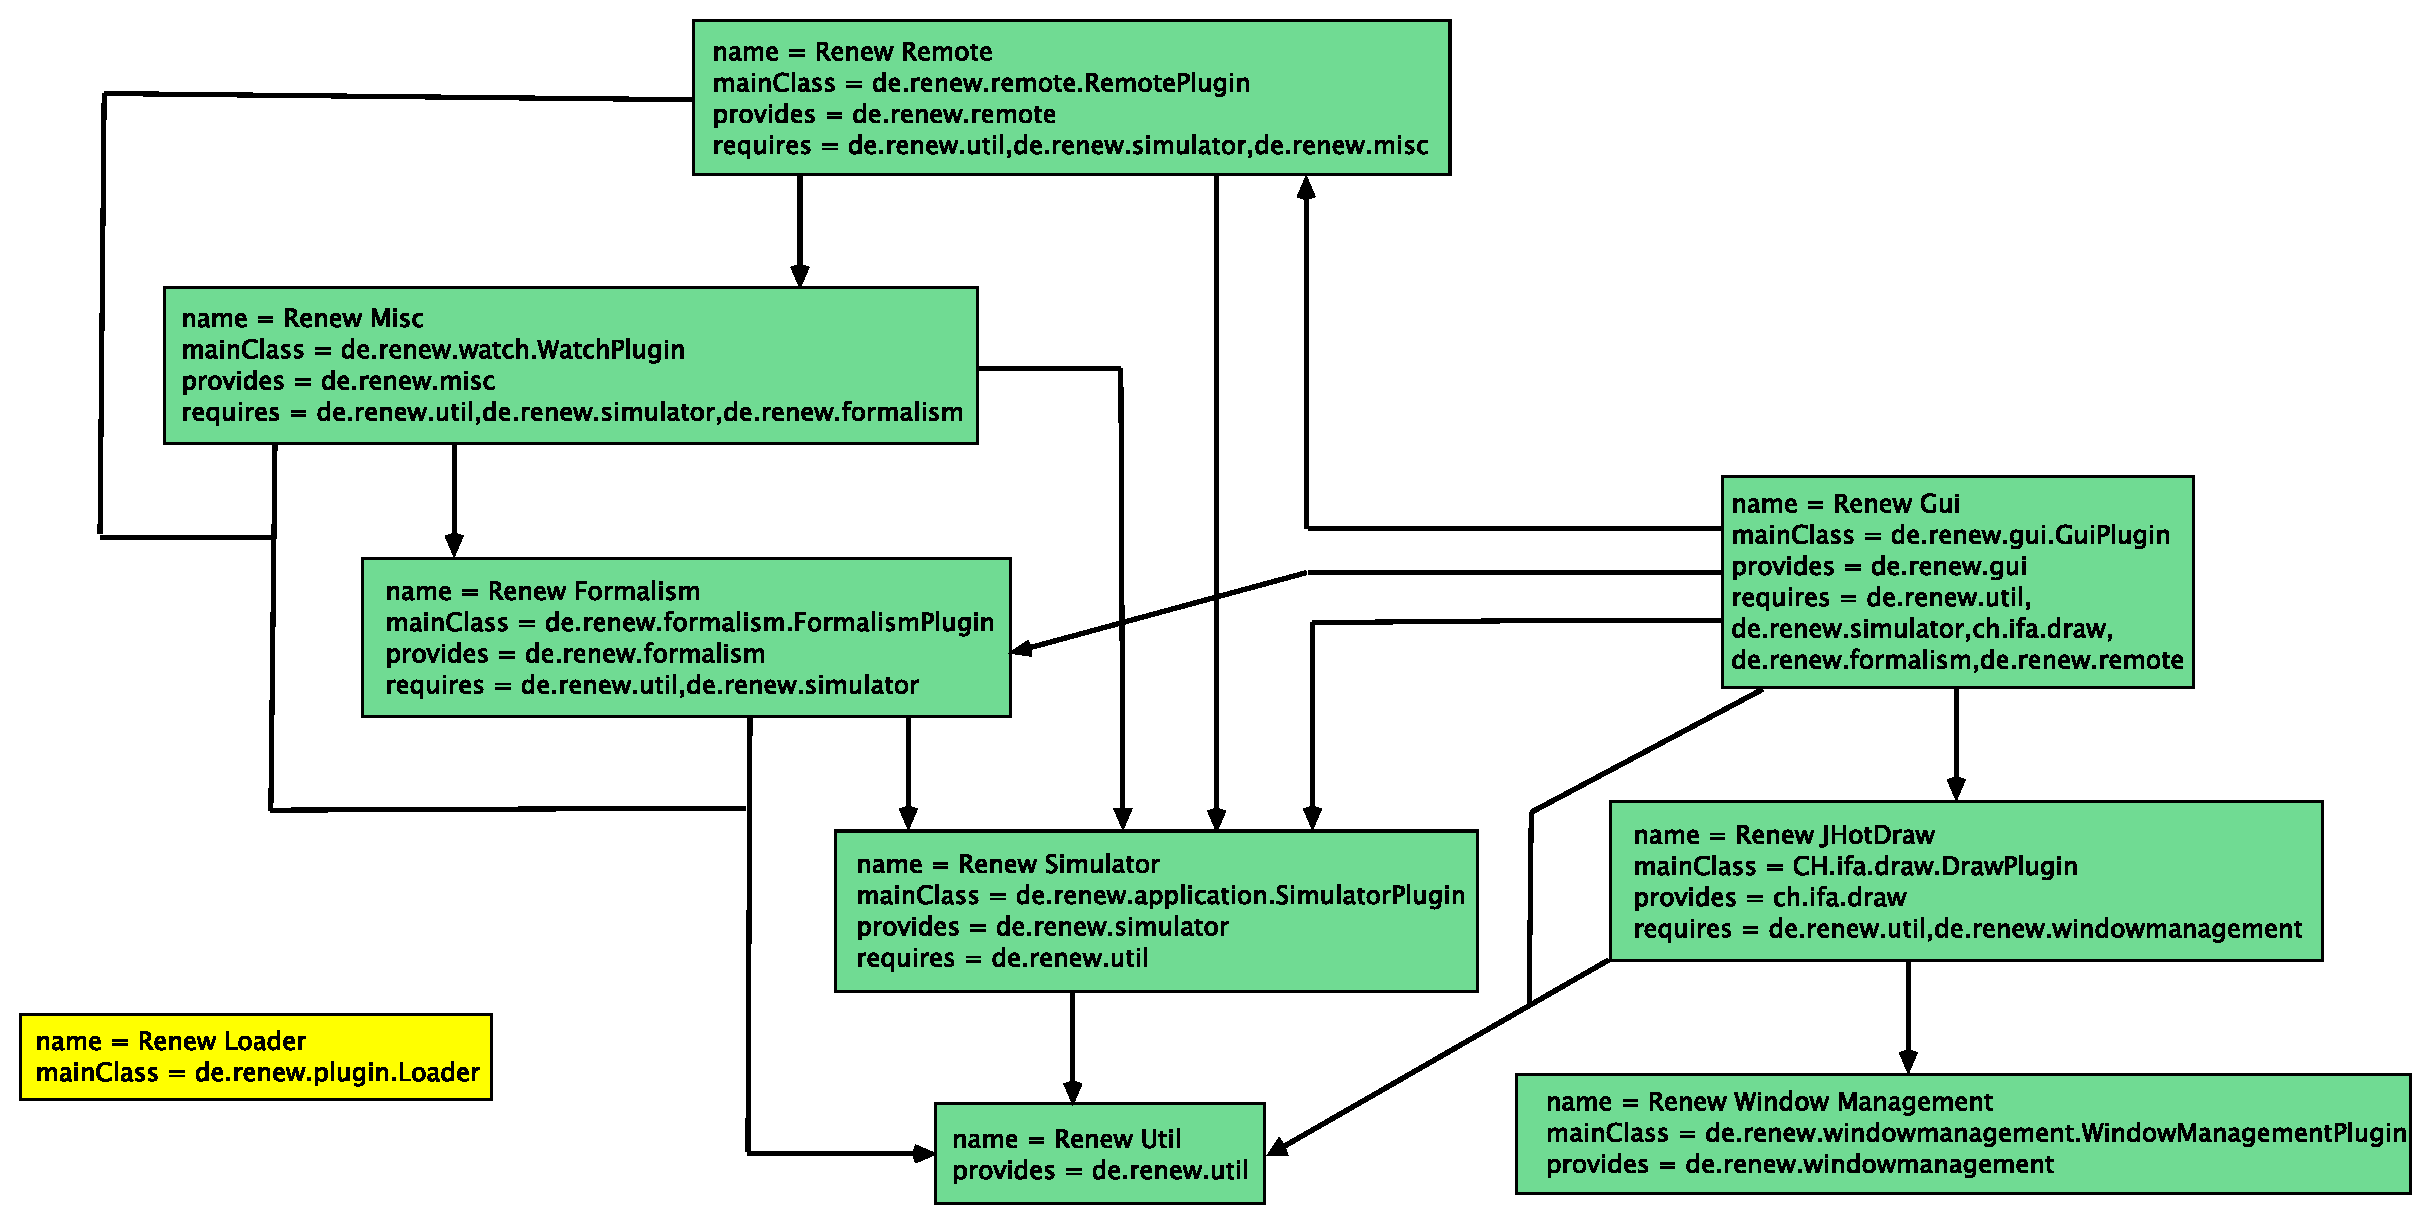
\includegraphics[width=\textwidth]{material/images/renew_plugin_dependencies2.pdf}
		  \caption{Gui Plugin-Abhängigkeiten}
		  \label{fig:plugin_deps}
		\end{figure}

		Für die Evaluation der minimalen Konfiguration starten wir aus dem \textit{Gui}-Plugin und arbeiten uns abwärts der Plugin-Hierarchie der \textit{plugin.cfg's} hinab, bis der komplette Graph aufgebaut ist.\newline

		Die in der Abbildung \ref{fig:plugin_deps} repräsentierten Zusammenhänge reflektieren die von den Entwicklern abgestimmten Laufzeitabhängigkeiten, die einen groben Überblick über die nötigen Plugins verschaffen. Diese können zur Laufzeit alle benötigten Daten und Klassen enthalten, jedoch tragen sie keine Aussage über Abhängigkeiten während der Kompilation. Demgemäß kann zusätzlicher Code sowie Plugins benötigt werden. 

	\subsection{Mulan} \label{sub:mulan}
		\textsc{Mulan} \cite{Roelke04} ist ein Multiagenten Rahmenwerk, mit dem Agenten entwickelt und miteinander verbunden werden können. Diese agieren nach eigenem Interesse und verhandeln über Kommunikationskanäle, die von \textsc{Mulan} angeboten werden. Um eine auf \textsc{Mulan} basierende Multi-Agent-Anwendung zu erstellen, müssen zahlreiche Protokollnetze gezeichnet und Wissensbasen erstellt werden, die das Verhalten und die Interaktion von Agenten implementieren. Somit bietet \textsc{Mulan} eine Kommunikationsplattform sowie ein Gerüst für die Umsetzung der darauf aufsetzenden Agenten und dessen Eigenschaften sowie Fähigkeiten, die mit Referenznetzen entworfen werden können. \cite{Cabac10a} \bigbreak

		Das Spiel Settler ist mit \textsc{Mulan} umgesetzt und implementiert somit die Agenten Anforderungen des Multi Agenten Systems. Diese halten Wissensbasen über die Spielregeln und können mit Hilfe der Protokollnetze bestimmte Entscheidungen treffen und Handlungen ausführen. Wie zum Beispiel Straßen bauen oder mit Karten handeln.\bigbreak
		
		\begin{figure}[h!]
		  \centering
		  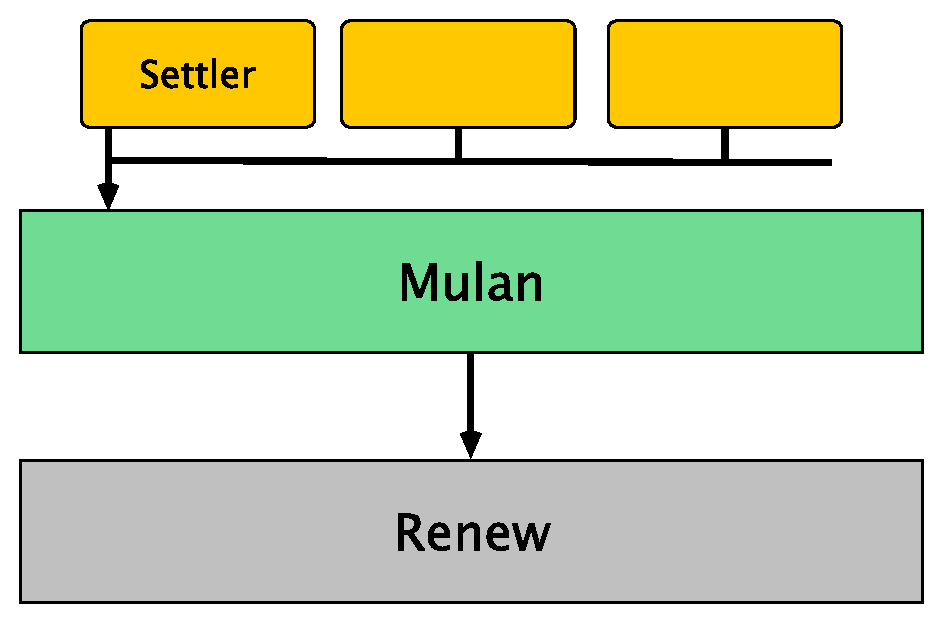
\includegraphics[width=0.5\textwidth]{material/images/settler-mulan-renew.pdf}
		  \caption{\textsc{Mulan} Plugins}
		  \label{fig:mulan_plugin}
		\end{figure}

		Damit die erstellten Settler Agenten und dessen Aufbau simuliert werden können, wird der \textsc{Renew} Petrinetz Simulator verwendet, mit dem die umgesetzten Agenten-Strukturen betrieben werden können.\newline
		Des Weiteren besitzt das Settler Spiel sowie das \textsc{Mulan}-Rahmenwerk eine Plugin konforme Architektur und werden somit genauso, wie die \textsc{Renew} Plugins von dem \textsc{Renew} Plugin-Manager ausgelesen und verwaltete.\bigbreak

		Ein vereinfachter Zusammenhang ist in der Abbildung \ref{fig:mulan_plugin} dargestellt und visualisiert die benötigten Grundlagen für die Ausführung von Settler.

\section{Durchführung} \label{sec:durchführung}
	Die wichtigen Szenarien für das Erreichen des gesetzten Ziels werden mit zwei Prototypen umgesetzt. Der \textsc{Renew} Prototyp wird eine kontinuierliche  Modularisierung der Plugins und dessen Betriebsfähigkeit mit nur zum Teil Modularisierter Codebasis abdecken. Dazu gehört das Erstellen einer neuen Projektstruktur für die auserwählten Plugins und behandelt auserwählte Richtlinien, die mit dem Modulsystem von Java eingeführt worden sind. Für das Anfertigen von ausführbar Code, wird das Gradle Werkzeug integriert, das einen Kompilation Kontext für die neuen Module erstellt. Dazu gehört eine Abhängigkeitsverwaltung sowie Projektkopplung. Um die Plugins mit einender als Module zu verzahnen, werden Schnittellen untersucht und in der \textit{module-info} Konfigurationsdatei in den Plugins verankert. In der folgenden Evaluation wird das Ergebnis evaluiert und sauber Aufbereitet.\bigbreak 

	Im Gegensatz dazu behandelt der \textsc{Mulan} Prototyp die Zusammenführung bestehender Systeme mit modularisiertem Code. Für die Umsetzung werden nur für das Spiel Settler relevanten \textsc{Mulan} Plugins erarbeitet und auf die minimale \textsc{Renew} Version aufgesetzt. Doch zuerst muss eine erweiterte Analyse der minimalen \textsc{Renew} Version durchgeführt werden, um die benötigten \textsc{Renew} Plugins für das \textsc{Mulan} Rahmenwerk nachzurüsten. Im weiteren Verlauf behandelt dieser Prototyp Konsequenzen der Umstellung auf eine neue \textsc{Renew} Grundlage und der benötigten Ausführungsschritte für die Adaption. Die Evaluation bewertet den Aufwand für die Umsetzung des Prototypen. 



%		- Plugin Gruppen verwalten ist in sich eine Herausforderung, da jedes Plugin kritisch für die Ausführung ist. 
%		- Module verwalten wird noch wichtiger. 
%		- Die Codebasen für unterschiedliche Module muss innerhalb und außerhalb(globale Einstellungen und Abhängigkeiten) eines Plugins verwaltet werden
%		- Eine saubere Struktur ist das Schlüsselkriterium 
%		- Die Module müssen sich gegenseitig kennen und dynamisch Zusammensetzbar sein.
%		- Kontrolliertes Ausrollen der Module ist wichtig für Renew, daher ist ein unterstützendes Tool willkommen.
%		- Diese muss Plugins auf Basis komplexer globaler Entscheidungen konstruieren. 
%		- Daher muss das Tool flexibel gesonderte Aufgabenstellungen umsetzen und bei Bedarf die Meta-Inforamtio der Plugins bearbeiten. 
%		- Dynamische Klassennamen Änderung ist möglich. (Es wird bereits Klasse Generiert basierend auf irgend etwas, jetzt können passende Module referenziert erstellt werden basierend auf etwas) 


 %	Die saubere Umsetzung behandelt den internen Aufbau, Namen- und Paketkonventionen sowie die Modulschnittstellen, die das Interagieren mit den Modulen einheitlich beschreiben und einen Vertrag mit den Nutzer eingehen. Zusätzlich muss der Inhalt eines Moduls klar festgelegt werden, da dieser nur einen Teil der zusammengesetzte Software abbildet und den Funktionsumfang beschränkt. \bigbreak 

 %Es müssen neue Konzepte integriert, Richtlinien befolgt und veraltete Konstrukte ersetze werde. Zu den genannten Problemen gehören Zyklen, Split-Packages und interne API-Zugriffe, die für den Umstieg sorgfältig gepflegt werden müssen.